\section{Teoría de Acoplamiento}
\label{sc:coupling_theory}

\subsection{Modelo Teórico de Anillo Resonador}

En la figura \ref{fig:rr_model} se muestra el esquema del caso genérico de 
un anillo resonador con 2 regiones de acoplamiento representadas 
por las líneas punteadas. 
Por simplicidad, el modelo asume que no hay pérdidas por 
acoplamiento (\ref{eq:energy_conserv}) y se ignoran los efectos de reflexión 
dentro de la guía (sólo se asumen ondas en el sentido de la propagación). 
El modelamiento teórico es muy similar al resonador Fabry-Perot descrito en
\cite{verdeyen1989laser}.

Cada región del anillo tiene asociados unos parámetros principales que definen su 
comportamiento. Estos son:
\begin{itemize}
\item Coeficientes de acoplamiento $(\kappa_1,\kappa_1^{'}\kappa_2\kappa_2^{'})$,
\item Coeficientes de transmisión $(t_1, t_1^{'}, t_2, t_2^{'})$ (en la sección 
\ref{ss:params_relation} se verá la relación que existe entre los 8 coeficientes). 
\item Constante de propagación $\beta$ del modo circulante. 
\begin{equation}
\beta=\frac{2 \pi}{\lambda} n_{eff}
\label{eq:beta}
\end{equation} 
Valor complejo donde $\Re\{\beta$\} es la constante de fase 
y $\Im\{\beta$\} representa las pérdidas por propagación
dentro del anillo.
\item Radio $r$ y perímetro $(L=2 \pi r)$ del anillo.
\end{itemize} 


\begin{figure}[h!]
\caption{Modelo de un Anillo Resonador}
\centering
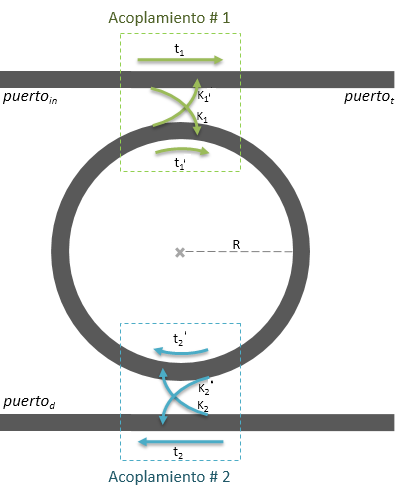
\includegraphics[width=0.7\textwidth,natwidth=396,natheight=495]{figs/rr_model.PNG}
\label{fig:rr_model}
\end{figure} 

Para que el dispositivo entre en resonancia, el desfase de la onda después de un viaje
completo al rededor del anillo debe ser un múltiplo entero de $2 \pi$

\begin{equation}
\beta L = 2 \pi M
\label{eq:resonant_condition}
\end{equation} 
 
Donde $M$ es llamado el número de modo (Figura \ref{fig:resonant_modes}). 

La potencia de la onda que se ve en el $puerto_t$ está dada por la porción de la onda incidente
que atravieza la guía más las $N\to\infty$ contribuciones que se dan por la otra parte de la
onda que se acopló en el anillo (ec. \ref{eq:coupling_gral}). 
Cada una de las contribuciones depende del número de viajes completos que realice la onda
acoplada antes de volver a salir a la guía superior.


\begin{equation}
E_t = E_i t_1 + Contrib_{M=1L} + Contrib_{M=2L} + ... + Contrib_{M=\infty L}
\label{eq:coupling_gral}
\end{equation} 

\begin{itemize}
\item Contribución después de una vuelta: $Contrib_{M=1L}$
\end{itemize} 


\begin{figure}[h!]
\caption{Contribución Onda 1 Vuelta}
\centering
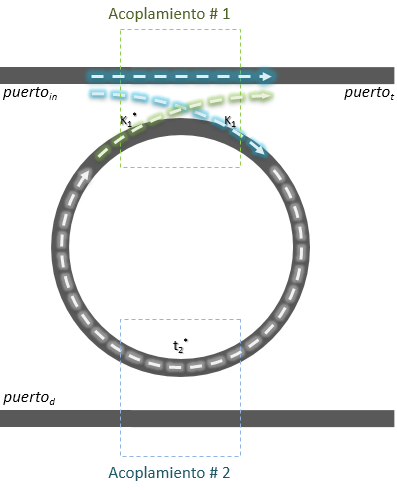
\includegraphics[width=0.7\textwidth,natwidth=397,natheight=490]{figs/rr_n1.PNG}
\label{fig:rr_n1}
\end{figure} 

El fasor escalar $\alpha e^{-j \beta L}$ contiene la información sobre la amplitud de
la atenuación debido a efectos de dispersión y a la curvatura de la onda 
($\alpha=1$ si no hay pérdida)
y la fase de la onda que ha recorrido una distancia L. 
Por lo tanto, al dar una vuelta ($1L$), la propagación de la onda queda expresada como 
$\alpha e^{-j \beta L}$.

En su recorrido completo, la onda que da una vuelta completa (Figura \ref{fig:rr_n1}) 
pasa por 3 regiones de interés. 
En la primera región (acoplamiento 1) una porción (dada por el coeficiente de acoplamiento 
$\kappa_1$) entra desde la guía recta hacia el anillo.
En la segunda región (acoplamiento 2), una porción (proporcional al coeficiente de transmisión 
$t_2^{'}$) continúa su viaje al interior del anillo.
Finalmente, en la tercera región (acoplamiento 1) sólo una parte de la onda 
(coeficiente de acoplamiento $\kappa_1^{'}$) vuelve a la guía original para 
salir por el $puerto_t$. 


Teniendo en cuenta cada una de estas atenuaciones más el fasor que expresa la propagación
de la onda, se llega a (\ref{eq:coupling_round_1}).

\begin{equation}
Contrib_{M=1L} = E_i \alpha e^{-j \beta L} \kappa_1 t_2^{'} \kappa_1^{'}
\label{eq:coupling_round_1}
\end{equation} 

\begin{itemize}
\item Contribución después de dos vueltas: $Contrib_{M=2L}$
\end{itemize} 

Se analizará la parte de la onda que no se reintegró a la guía recta tras la primera vuelta
y que da otra vuelta antes de volver a la guía recta para salir por el $puerto_t$
(Figura \ref{fig:rr_n2}).
La propagación de la onda tras 2 vueltas completas ($2L$), está dada por 
$\alpha^2 e^{-j \beta 2L}$.
La onda atravieza 2 nuevas regiones (aparte de las 3 regiones mencionadas en la sección anterior)
por cada nueva vuelta que deba dar. 

La primera es la región de acoplamiento 1 (en una proporción dada por $t_1^{'}$) 
para seguir su trayectoria dentro del anillo.
La segunda es la región de acoplamiento 2, la cual debe atravezar (según el factor de 
transmisión $t_2^{'}$).

Estas nuevas atenuaciones se ven reflejadas en (\ref{eq:coupling_round_2}). 
El término $\alpha^2 e^{-2j \beta L}$ se expresó como
 $\alpha e^{-j \beta L} \alpha e^{-j \beta L}$ para facilitar
su generalización posterior.

\begin{figure}[h!]
\caption{Contribución Onda 2 Vueltas}
\centering
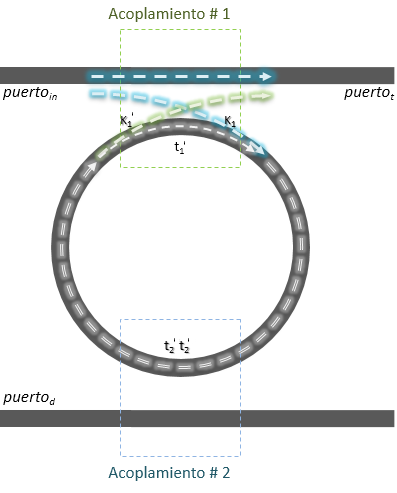
\includegraphics[width=0.7\textwidth,natwidth=397,natheight=493]{figs/rr_n2.PNG}
\label{fig:rr_n2}
\end{figure} 

\begin{equation}
Contrib_{M=2L} = E_i \alpha e^{-j \beta L} \kappa_1 t_2^{'} \kappa_1^{'} (\alpha e^{-j \beta L} t_1^{'} t_2^{'})
\label{eq:coupling_round_2}
\end{equation} 

\begin{itemize}
\item Contribución después de N vueltas: $Contrib_N$
\end{itemize} 

Por cada vuelta adicional antes de acoplarse, se deben tener en cuenta los 
coeficientes de transmisión en estas 2 regiones más el desfase y la atenuación de la 
onda en cada vuelta (\ref{eq:coupling_round_n}).

\begin{equation}
Contrib_N = E_i \alpha e^{-j \beta L} \kappa_1 t_2^{'} \kappa_1^{'} (\alpha e^{-j \beta L} t_1^{'} t_2^{'})^{N-1}
\label{eq:coupling_round_n}
\end{equation} 

Sustituyendo la expresión para cada una de las contribuciones en 
(\ref{eq:coupling_gral}) y reorganizando, se llega a (\ref{eq:coupling_sum}).


\begin{equation}
E_t = E_i\{
t_1+
\kappa_1\kappa_1^{'} t_2^{'} \alpha e^{-j \beta L} [
1 +
(t_1^{'} t_2^{'} \alpha e^{-j \beta L})^1 +
(t_1^{'} t_2^{'} \alpha e^{-j \beta L})^2 +
...]\}
\label{eq:coupling_sum}
\end{equation}

Al ser una serie geométrica infinita, su solución está dada por (\ref{eq:geom_series}).

\begin{equation}
\sum\limits_{k = 0}^\infty {ar^{k} = \frac{a}{{1 - r}}}, \text{ si } |r| < 1
\label{eq:geom_series}
\end{equation} 

Sea 
$a = \kappa_1 \kappa_1^{'} t_2^{'} \alpha e^{-j \beta L} $ y  
$r = t_1^{'} t_2^{'} \alpha e^{-j \beta L}$.
Por lo tanto:

\begin{subequations}
\begin{align}
E_t &= E_i\{t_1 + 
\frac{ \kappa_1 \kappa_1^{'} t_2^{'} \alpha e^{-j \beta L}}
{1 - t_1^{'} t_2^{'} \alpha e^{-j \beta L}} \} \\
\frac{E_t}{E_i} &= 
    \frac{t_1 + (\kappa_1 \kappa_1^{'} - t_1 t_1^{'})t_2^{'} \alpha e^{-j \beta L}}
    {1 - t_1^{'} t_2^{'} \alpha e^{-j \beta L}}
\label{eq:t_through}
\end{align} 
\end{subequations}

El cálculo de la potencia transmitida en el $puerto_d$ (\ref{eq:t_drop}) sigue una
lógica similar.

\begin{equation}
\frac{E_d}{E_i} = \frac{ \kappa_1 \kappa_2^{'} \alpha e^{ -j \beta \frac{L}{2}} }
	   { 1 - t_1^{'} t_2^{'} \alpha e^{-j \beta L} }
\label{eq:t_drop}
\end{equation} 

\subsection{Relación entre Coeficientes de Acoplamiento}
\label{ss:params_relation}

Como se explica en \cite{yariv2006photonics}, los 4 coeficientes de transmisión más
los 4 coeficientes de acoplamiento no son independientes entre si, sino que están
relacionados por los principios fundamentales de reciprocidad, conservación de la energía
y T-simetría. Adicionalmente, como se mencionó en el apartado anterior, el sistema
asume que no hay pérdidas por inserción (\ref{eq:energy_conserv}). 

\begin{subequations}
\begin{equation}
|t_1|^2 + |\kappa_1|^2 = 1  \label{eq:energy_conserv} 
\end{equation} 
\begin{equation}
t_1 t_1^{'} - \kappa_1 \kappa_1^{'} = -1 \label{eq:unitary_matrix} 
\end{equation} 
\begin{equation}
t_i = |t_i|e^{j \phi_{t_i}} \label{eq:t_coef}
\end{equation} 
\end{subequations}

Por conveniencia, en \cite{yariv2006photonics} se define el sistema 
del acoplamiento 1 mediante una matriz Hermitiana
(\ref{eq:hermitian_system}) con determinante -1. 
Esto permite relacionar facilmente el coeficiente de transmisión dentro 
del anillo $t_1^{'}$ en términos de la conjugada 
compleja del coeficiente de transmisión $t_1$.

\begin{equation}
    \left[ \begin{array}{c} E_s \\ E_{sk} \end{array} \right] 
    =
    \begin{bmatrix} t_1 & k_1^* \\ k_1 & -t_1^* \end{bmatrix} 
    \left[ \begin{array}{c} E_i \\ E_{ik} \end{array} \right]
\label{eq:hermitian_system}
\end{equation} 

Por comparación directa de (\ref{eq:hermitian_system}) con el sistema inicial, 
se ve que $t_1^{'} = -t_1^*$ y $t_2^{'} = -t_2^*$.
Reemplazando estas equivalencias y  
(\ref{eq:unitary_matrix}) en (\ref{eq:t_through}) se encuentra la
expresión para la amplitud normalizada en el $puerto_t$ (\ref{eq:t_through_simp}).

\begin{align}
\frac{E_t}{E_i} &= 
    \frac{t_1 - t_2^* \alpha e^{-j \beta L}}
    {1 - t_1^* t_2^* \alpha e^{-j \beta L}} \label{eq:t_through_simp}
\end{align} 

Cuya función de transmisión (\ref{eq:T_t}) obtenida al multiplicar
por la correspondiente conjugada compleja (recordar que $|\chi|^2 = \chi \chi^*$)
es \cite{paloczi2005polymer}:

\begin{align}
 T_t &= \abs*{\frac{E_t}{E_i}}^2 = 
    \frac{\alpha^2 |t_2|^2 + |t_1|^2 - 2\alpha |t_1||t_2| 
	\cos(\theta + \phi_{t_1} + \phi_{t_2}) }
    {1 + \alpha^2|t_1|^2 |t_2|^2 - 2\alpha |t_1||t_2|
	\cos(\theta + \phi_{t_1} + \phi_{t_2}) }
\label{eq:T_t}
\end{align} 

Donde $\theta = \beta L = \frac{2\pi n_{eff}}{\lambda} L$. Para el $puerto_d$, se calcula la amplitud normalizada a partir de (\ref{eq:t_drop}) como:

\begin{equation}
\frac{E_d}{E_i} = \frac{ \kappa_1 \kappa_2^* \alpha e^{ -j \beta \frac{L}{2}} }
	   { 1 - t_1^* t_2^* \alpha e^{-j \beta L} }
\label{eq:t_drop_simp}
\end{equation} 

De (\ref{eq:t_drop}) y (\ref{eq:energy_conserv}) se obtiene también su función de
transmisión \cite{abujnah2012numerical}:

\begin{align}
 T_d &= 
    \frac{\alpha^2 (1-|t_1|^2) (1-|t_2|^2)}
    {1 + \alpha^2|t_1|^2 |t_2|^2 - 2\alpha |t_1||t_2|
	\cos(\theta + \phi_{t_1} + \phi_{t_2}) }
\label{eq:T_d}
\end{align} 

\subsection{Filtro Notch}
\label{ss:notch}

Un caso especial de (\ref{eq:t_through_simp}) se da cuando la onda es 
transmitida completamente dentro del anillo resonador en la región de acoplamento 2 \cite{yariv2006photonics}. 
En este caso $t_2^* = 1$ y $k_2^* = 0$ por lo que la salida en el $puerto_d$ es cero y
en el $puerto_t$ es (\ref{eq:t_through_notch}).
El sub-índice de $t_1$ no es necesario ya que sólo hay un acoplamiento.

\begin{subequations}
\begin{equation}
    \frac{E_t}{E_i} = 
	\frac{t - \alpha e^{-j \beta L}} {1 - t^* \alpha e^{-j \beta L}} 
\label{eq:t_through_notch} 
\end{equation}
\begin{equation}
     T_t = \frac{\alpha^2 + |t|^2 - 2\alpha |t| \cos(\theta + \phi_t) }
             {1 + \alpha^2|t|^2 - 2\alpha |t| \cos(\theta + \phi_t) }
\label{eq:T_t_notch}
\end{equation} 
\end{subequations}

\subsubsection{Acoplo Crítico}

Se observa que ocurre una situación especial cuando la suma de los desfases que
sufre la onda en su viaje completo al rededor del anillo es un múltiplo entero
de $2\pi$ (\ref{eq:resonance_condition}). 
Esta condición es llamada condición de resonancia (Figura \ref{fig:resonant_modes}).

\begin{equation}
\theta + \phi_t = 2\pi * M
\label{eq:resonance_condition}
\end{equation} 

\begin{figure}[h!]
\caption{Modos Resonantes. Fuente\cite{blasco2011desarrollo}}
\centering
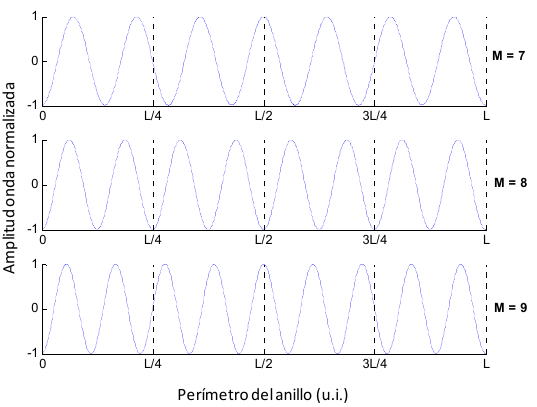
\includegraphics[width=0.8\textwidth,natwidth=537,natheight=437]{figs/resonant_modes.png}
\label{fig:resonant_modes}
\end{figure} 

Bajo esta condición, la ecuación de transmisión en el $puerto_t$ queda:
\begin{equation}
T_t=\frac{(\alpha - |t|)^2}{(1-\alpha|t|)^2}
\label{eq:t_resonance}
\end{equation} 

A partir de (\ref{eq:t_resonance}) se ve que cuando $\alpha=|t|=\sqrt{1-|\kappa|^2}$ la transmitancia
en el $puerto_t$ es cero. Es decir que cuando las pérdidas en la región de 
acoplamiento son iguales a las pérdidas en el anillo, se llega a la condición
llamada Acoplo Crítico, donde la potencia de salida se anula.

Visto desde el punto de vista de \cite{blasco2011desarrollo} el fenómeno se 
produce porque la longitud de onda que cumple la condición se acopla, sufre un 
desfase de $\frac{\pi}{2}$, es decir $\kappa = i|\kappa|$. 
Luego de completar una vuelta completa sufre un desfase de $2\pi$ y cuando
se vuelve a acoplar a la guía recta es desfasada nuevamente $\frac{\pi}{2}$.
Es decir, que cuando vuelve a la guía inicial, se suma en contrafase en el 
punto de acoplamiento de la guía, anulándola.

\subsection{Parámetros}

Existen diferentes parámetros que son relevantes a la hora de describir el rendimiento
de un anillo resonador. A continuación se realizará la formulación matemática de 
cada uno acompañado de una breve descripción.

Los parámetros para el notch filter se obtienen sustituyendo $t_2$ por 1, como se explicó en
la sección \ref{ss:notch}.

\subsubsection{Free Spectral Range (FSR)}
El FSR o rango libre de espectro, es la separación que existe entre dos longitudes
de onda que resuenan dentro del anillo. De (\ref{eq:resonant_condition}) y
(\ref{eq:beta}) se tiene que:

\begin{align}
M&=\frac{n_{eff_{(\lambda_m)}} L}{\lambda_m} \label{eq:mode_l} \\
M+1&=\frac{n_{eff_{(\lambda_{m+1})}} L}{\lambda_{m+1}} \label{eq:mode_l+1}
\end{align} 

La constante de propagación no es constante debido a la dispersión dentro de la guía por lo que 
se usa en índice de grupo (\ref{eq:ng}) en vez de el índice efectivo \cite{paloczi2005polymer}.

\begin{equation}
n_g=n_{eff} - \lambda \frac{\partial n_{eff}}{\partial \lambda}
\label{eq:ng}
\end{equation} 

El FSR, dado por $\Delta \lambda=\lambda_{m+1}-\lambda_m$ se halla restando
(\ref{eq:mode_l+1}) y (\ref{eq:mode_l}). También se 
asume que $n_{eff_{(\lambda_m)}} \approx n_{eff_{(\lambda_{m+1})}} \approx M $ 
y que $\lambda_m \lambda_{m+1} \approx \lambda^2 $, por lo tanto:

\begin{equation}
FSR=\Delta \lambda \approx \frac{\lambda^2}{n_g L}  
\label{eq:fsr}
\end{equation} 


De (\ref{eq:fsr}) se puede observar que el FSR es inversamente proporcional a el 
radio del resonador. Para un anillo con un radio grande el distanciamiento
entre las longitudes de onda que resuenan en él es menor. Esto indica su capacidad
para manejar una densidad de espectro alta y son principalmente usados como switches
de bada ancha. 

Por el otro lado, un anillo pequeño tendrá un mayor espaciamiento
entre los modos lo que significa que es más selectivo \cite{chan2011physical} y por
eso son muy usados como filtros y moduladores.

\subsubsection{Full Width Half Maximum}

La anchura a media altura representa el ancho de la resonancia
medido en nanómetros $(\Delta \lambda_{FWHM})$ cuando ésta 
decae 3dB o mitad de la potencia y su expresión
para una cavidad Fabry-Perot \cite{paloczi2005polymer}\cite{verdeyen1989laser} es:

\begin{equation}
\Delta \lambda_{FWHM}=2\delta \lambda
    =\frac{\lambda_0^2}{L n_{eff} \pi} 
     \left( \frac{1-\alpha^2|t_1|^2|t_2|^2}{\alpha |t_1||t_2|}  \right)
\label{eq:fwhm}
\end{equation} 

\subsubsection{Quality Factor (Q)}

El factor de calidad es una relación entre la longitud de onda que resuena en el 
anillo y el ancho de la resonancia en la mitad de la potencia.

\begin{equation}
Q = \frac{\lambda_0}{\Delta \lambda_{FWHM}} 
  = \pi \frac{n_{eff} L}{\lambda_0} \frac{\alpha|t_1||t_2|}{1-\alpha^2|t_1|^2|t_2|^2}
\label{eq:q}
\end{equation}

\subsubsection{Finesse (F)}

La finura F permite medir la estrechez de las resonancias \cite{blasco2011desarrollo},
donde entre más estrecha, el anillo es más selectivo.

\begin{equation}
F=\frac{FSR}{\Delta \lambda_{FWHM}}
 =\frac{\Delta \lambda}{2 \delta \lambda} 
 = \pi \frac{\alpha|t_1||t_2|}{1-\alpha|t_1|^2|t_2|^2}
\label{eq:finesse}
\end{equation} 

En (\ref{eq:finesse}) se aprecia que entre menos pérdidas existan en el anillo, 
la finura del anillo es más elevada.

 
